\subsection{写真撮影画面}
写真撮影画面ではiPhoneに内蔵しているカメラを使用して現地の写真を撮影する。カードリスト画面で木古内の魅力を知り、実際に現地へ訪れたユーザにそこへ訪れた証拠を残してもらうために写真を撮ってもらう。撮った画像はカードリストの画像に上書きされ、表示される。写真撮影画面はカードリスト画面のカメラボタンをタップすることで画面遷移する。写真撮影画面が呼び出された画面を図6.4(a)で示す。画面の下の中心にある丸いボタンを押すと写真を撮ることができる。左下のキャンセルボタンを押すと写真撮影画面からカードリスト画面に画面遷移する。左上のボタンはフラッシュの有無を選択でき、暗い風景を撮るときなどに使用する。右上のボタンはインカメラとアウトカメラの切り替えを行うことができる。写真を撮ったらその画像を使用するか選択する写真保存画面に遷移する。写真保存画面はを図6.4(b)で示す。写真保存画面ではユーザが撮った写真が気に入った場合、右下の写真を使用ボタンを選択することでその写真は保存され、撮った場所のカードリストの画像に表示される。撮った写真が気に入らなかった場合は、左下の再撮影ボタンを押すことで写真撮影画面に戻ることができる。

\begin{figure}[htbp]
  \begin{center}
    \begin{tabular}{c}

      % 1
      \begin{minipage}{0.33\hsize}
        \begin{center}
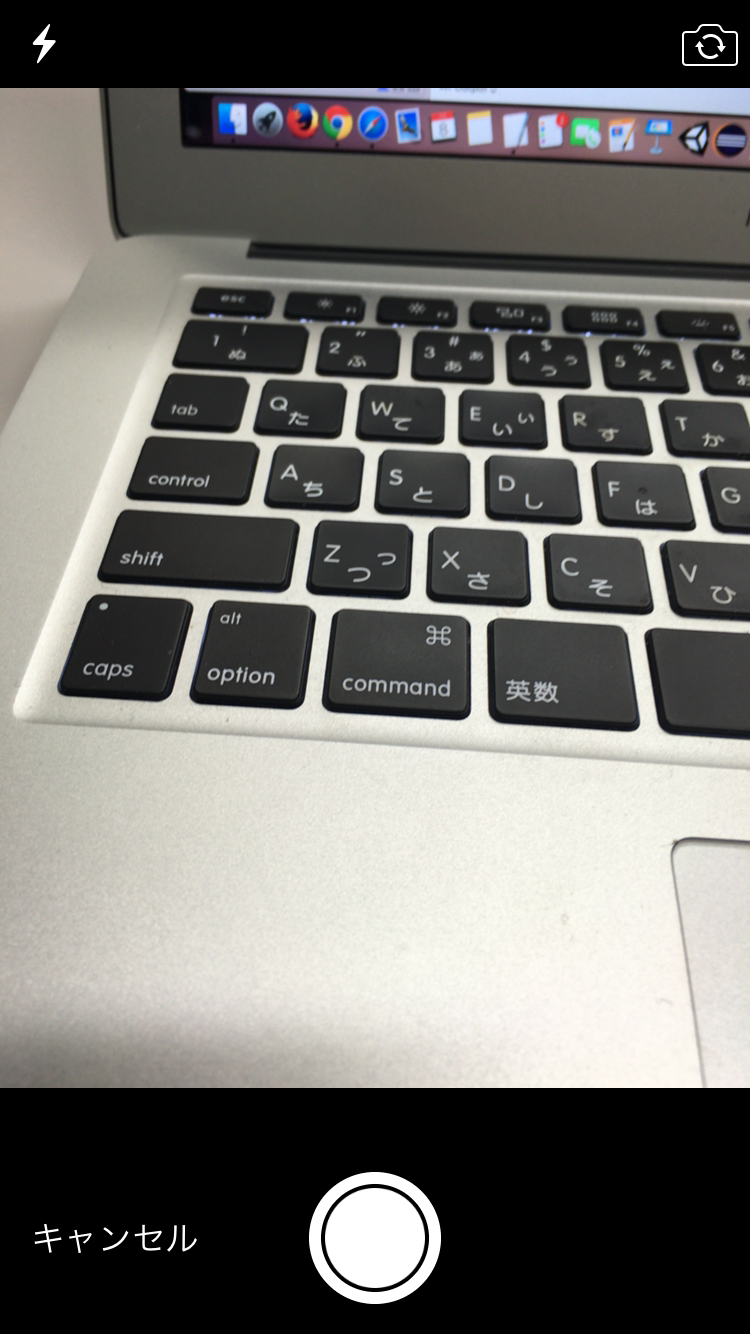
\includegraphics[width=4cm, bb=0 0 304 570]{kiko_takephoto1.PNG}
          \hspace{1cm} (a)写真撮影画面
        \end{center}
      \end{minipage}

      % 2
      \begin{minipage}{0.33\hsize}
        \begin{center}
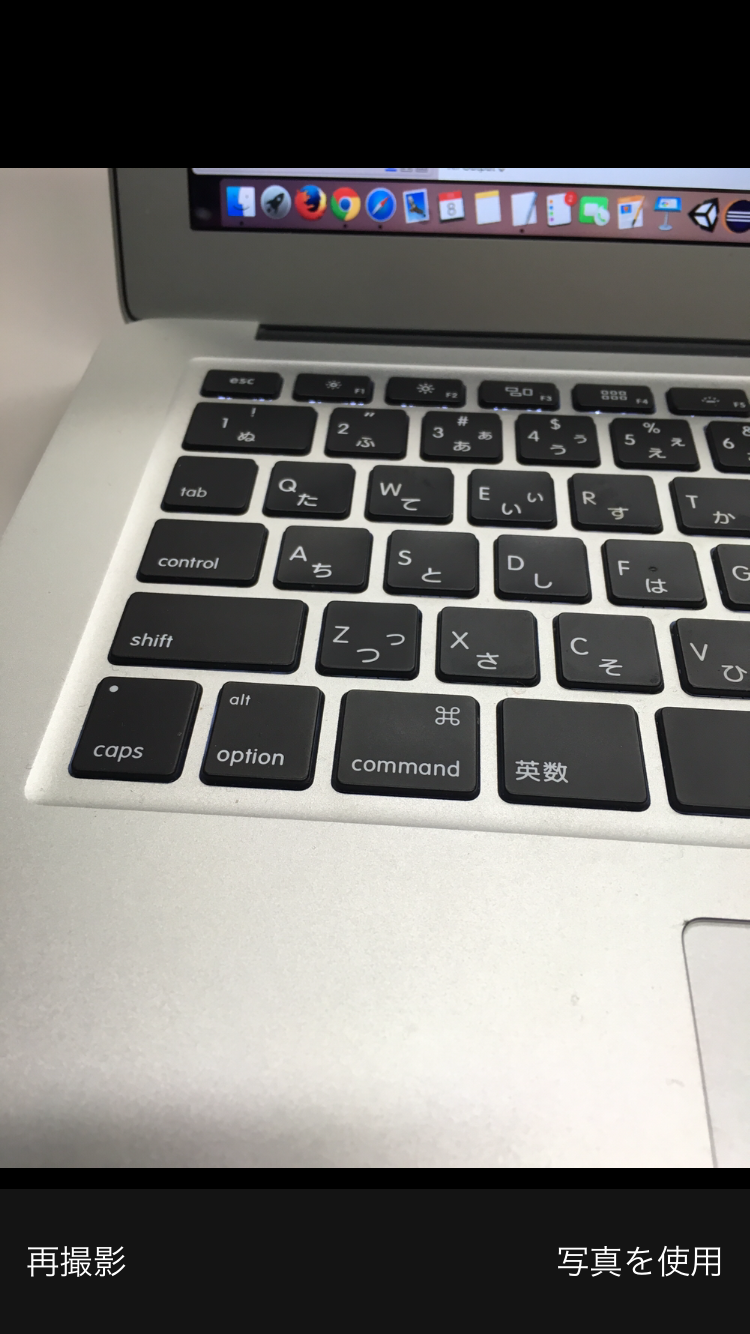
\includegraphics[width=4cm, bb=0 0 304 570]{kiko_takephoto2.PNG}
          \hspace{1cm} (b)写真保存画面
        \end{center}
      \end{minipage}
      
    \end{tabular}
    \caption{写真を撮影する機能の画面}
    \label{fig:lena}
  \end{center}
\end{figure}          

\bunseki{池田俊輝}